%% TODO: Clean up billeder
In order to demo our application, we first need to get it up and running.

\section{Getting the code}
There are two options in regards to getting our code up and running; either you
run it locally (and set it up yourself), or you run it remotely by utilizing
the system, that we've already setup.

Below we'll be going through both of these cases, starting with the more 
difficult local case, then moving on to the remote case.

\subsection{Running locally}
We've developed a docker image for our project, as such one can start the 
fake-dht backend server, and the \acs{HTTP}-server (serving our web-interface), using:
\begin{verbatim}
docker run -it -p 80:1987 -p 3000:3000 skeen/streamy
\end{verbatim}
After which the web-interface will be hosted on port 80, while the fake-dht,
will be running on port 3000. Assuming the docker instance is running locally,
one should be able to access the web-interface at: \url{http://localhost/}.

\subsection{Remotely}
\label{subsec:running-remotely}
We're running above mentioned docker image on a digital ocean server, as such
one can access the site by going to \url{http://skeen.info/}, or circumventing
DNS by going to \url{46.101.226.102}.

\section{Using the application}
At this point it's assumed that the system is up and running. If one is using 
the local setup, the \acs{DHT} will be empty, and no results will be found by
searching, while two results should pop up using the remote setup, namely;
\begin{itemize}
\item 'The Start': A chiptunes song by Tiasu
\item 'Pixelland': A chiptunes song by Kevin MacLeod
\end{itemize}
{\em Both of these songs are used with permission, and we've setup a node which will
be seeding them continuously, until the exams are complete.}

\subsection{Uploading songs / Populating the \acs{DHT}}
In order to add songs to the \acs{DHT}, they must be uploaded to the network, by 
dropping them over within the drag-and-drop field on the bottom of the page.
When a song is dropped here; it is added to the \acs{DHT}, saved to local storage,
and then it's seeded by the browser for others to download.

\subsection{Acquiring content}
At this point it's assumed that the \acs{DHT} is populated, and that a seed for the
content is available. It's worth noting that the \acs{DHT} does not clear out dead
content, or otherwise decay entries, as \acs{DHT}s usually do, as such the \acs{DHT} can 
somewhat easily be brought to an inconsistent state, i.e. where the \acs{DHT}
contains content which does not have any seeds.
\newline\newline
At this point, one should be able to acquire information about a song from the
\acs{DHT}, by entering the title of a song in the search field (top right corner).
The search field features type-ahead, and whenever a suggestion is clicked,
detailed information about that content is displayed;

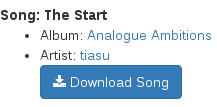
\includegraphics{gfx/search-info}
\newline
Clicking the artist or album, will look up their entries in the \acs{DHT}, and thus
provide detailed information about these. Clicking the 'Download Song' button,
will initialize the download, and add an entry to the download tab, which will
continuously update with information on the download process;

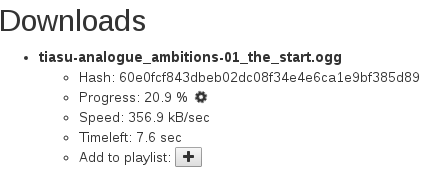
\includegraphics{gfx/download-info}
\newline
{\em It's preferable to use incognito mode, or different browsers for testing this,
as local storage is shared between tab, and may otherwise interfere.}
\newline\newline
Once the content is fully downloaded it'll move to the local tab, from which it
will be seeded and updated with seeding information. 

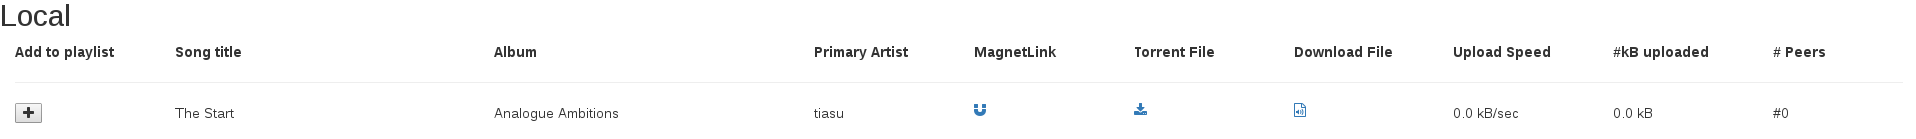
\includegraphics[width=\linewidth]{gfx/local-info}

\subsection{Playing back content}
The first step is playing back content, is to add the content to the play-list.
This can be done by using clicking one of the small plusses (+), on either the
local content tab, or the download tab.
\newline
After adding a song, one can double-click an entry in the play-list to start the
playback of that entry on the player at the top of the page.

Playing back from the downloads tab (i.e. playing back content, which is
currently downloading), setups the torrent in streaming mode, such that pieces
are download in the order they're needed, rather than in the typical
rarest-first order.
{\em Note that not all file formats can be streamed; streamability and playback
of different file formats is browser dependent, and given by the specific
implementation of the \acs{HTML}5 audio tag.}
\newline\newline
The player contains a variety of buttons, these are considered to be self
explanatory for anyone whom has used a media player before. Below is a full
screen-shot of our web-interface taken while playback of a local song is in
progress.

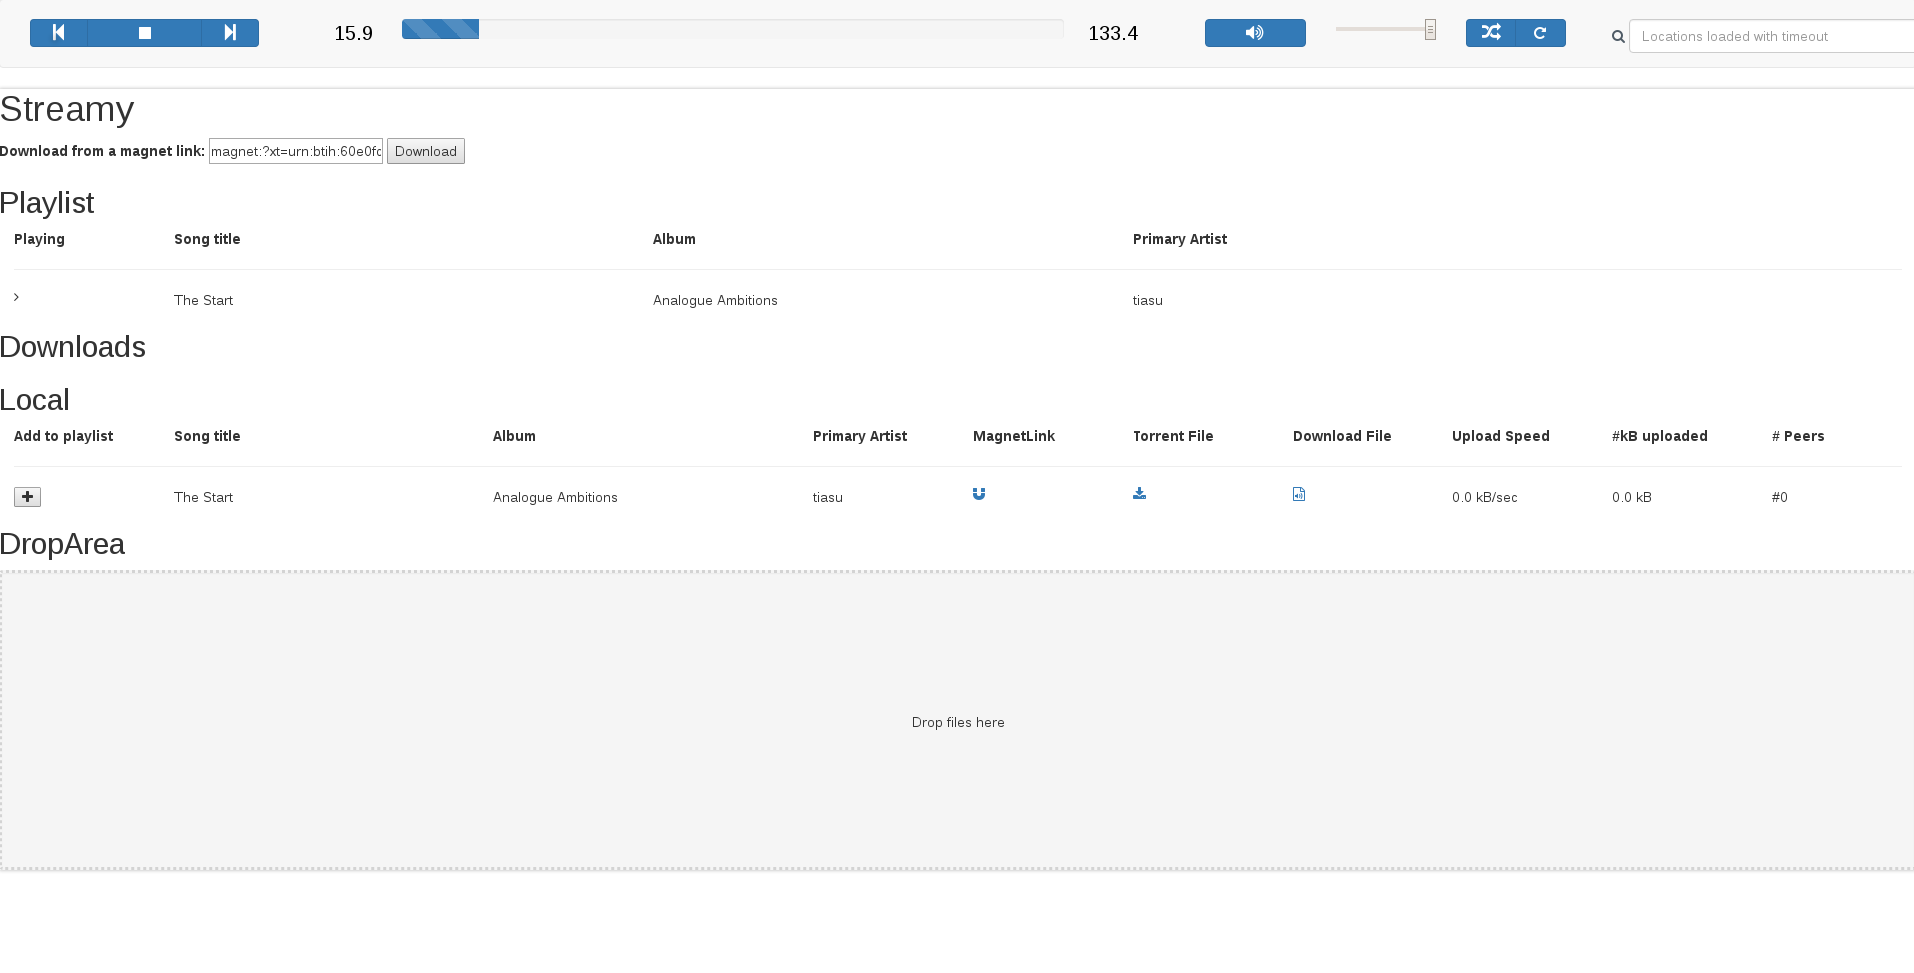
\includegraphics[width=\linewidth]{gfx/interface}
\newline
We encourage the reader to play around with the interface, including with the
features not documented here, such as downloading local-content to disk,
downloading by magnetURI, etc.
